\scanpage{35}
\margin{34}
\figure{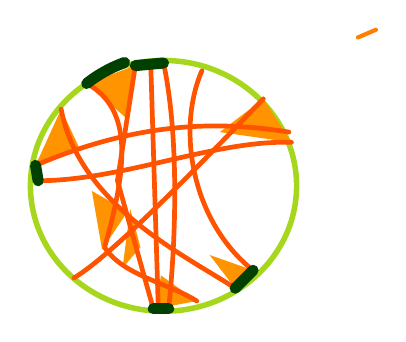
\begin{tikzpicture}[x=.65cm,y=.65cm,line cap=round,line join=round]
\draw[yellow!65!green,line width=2pt] (0,0) ellipse (2.6 and 2.45);
\fill[orange!85!yellow] (-1.5,2)--(-.7,1.3)--(-.55,2.35)--cycle;
\fill[orange!85!yellow] (-2.5,.4)--(-1.65,.75)--(-2,1.5)--cycle;
\fill[orange!85!yellow] (1.95,1.7)--(1.1,1.05)--(2.5,.85)--cycle;
\fill[orange!85!yellow] (-1.4,-.1)--(-.7,-.5)--(-1.2,-1.25)--cycle;
\fill[orange!85!yellow] (-.65,-.45)--(-.45,-1.2)--(-.8,-1.6)--cycle;
\fill[orange!85!yellow] (.65,-2.25)--(-.05,-1.75)--(-.15,-2.4)--cycle;
\fill[orange!85!yellow] (1.4,-2)--(.9,-1.35)--(1.75,-1.65)--cycle;
\draw[orange!65!red,line width=1.7pt] (-1.5,2) .. controls (-.6,1.5) and (-.7,.4) .. (-1.15,-1.2) .. controls (-.8,-1.75) and (.1,-1.9) .. (.65,-2.25);
\draw[orange!65!red,line width=1.7pt] (-.55,2.35)--(-.9,.1)--(-.2,-2.4);
\draw[orange!65!red,line width=1.7pt] (-.25,2.4)--(-.1,-2.45);
\draw[orange!65!red,line width=1.7pt] (0,2.4) .. controls (.3,1) and (.25,-1) .. (.1,-2.4);
\draw[orange!65!red,line width=1.7pt] (.75,2.25) .. controls (.25,1.1) and (.55,-.7) .. (1.75,-1.65);
\draw[orange!65!red,line width=1.7pt] (1.95,1.7) .. controls (.75,.45) and (-1,-1.35) .. (-1.75,-1.8);
\draw[orange!65!red,line width=1.7pt] (-2.45,.1) .. controls (-.8,.1) and (1,.9) .. (2.5,.85);
\draw[orange!65!red,line width=1.7pt] (-2.5,.4) .. controls (-.4,1.3) and (1.2,1.25) .. (2.45,1.05);
\draw[orange!65!red,line width=1.7pt] (-2,1.5) .. controls (-1.65,-.4) and (.5,-1.4) .. (1.4,-2);
\draw[green!25!black,line width=4pt] (-1.5,2) arc (130:111:2.6 and 2.45);
\draw[green!25!black,line width=4pt] (-.55,2.35)--(0,2.4);
\draw[green!25!black,line width=4pt] (-2.5,.4)--(-2.45,.1);
\draw[green!25!black,line width=4pt] (-.2,-2.4)--(.1,-2.4);
\draw[green!25!black,line width=4pt] (1.4,-2)--(1.75,-1.65);
\draw[orange,line width=1.5pt] (3.8,2.9)--(4.15,3.05);
\end{tikzpicture}}
On trouve un ``syst. de cordes'' \inserted{$d_i=(D_i)_L$} dans $\Delta=\Delta_L$ qui a les propriétés suivantes

a) Deux $d_i$ se coupent en au plus un point, lequel est \uline{intérieur} à $\Delta$, et elles se croisent en ce point.

(Cela fait partie de la notion $:=$ de ``syst de cordes'', \inserted{\unsure{déf°}} avec la condition que les $d_i$ soient des segments topologiques et $\partial d_i=d_i\cap\partial\Delta$)

b) La relation dans $I$ ``$i=j$ ou \deleted{$\unsure{d_i\ne d_j}$} $\delta_i\cap\delta_j=\varnothing$'' \deleted{est} (``parallélisme'') est une relation d'équivalence, et \deleted{\unsure{si l'on}} si on a une classe \deleted{\unsure{d'équivalence de $\nu$ éléments}} \inserted{d'équi. $C$, \deleted{\unsure{qui a plus}} $\nu\geq2$}, alors l'ensemble des \inserted{$2\nu$} sommets correspondants est réparti en 2 paquets \inserted{$S',S''$} de $\nu$, \deleted{\unsure{un}} [naturellement \inserted{\unsure{non-}}antipodiques] (NB cela a un sens rigoureusement combinatoire, les \unsure{bds $\partial\delta$} des segments du syst. étant une \unsure{paire})] \inserted{avec \deleted{\unsure{les}} $\delta\cap S'$ et $\delta\cap S''$ réduits à un point pour t\textsuperscript{t} $\delta\in C$}, et les sommets des ch. des deux paquets, forment vis à vis de $C$ fixe, $(s_1,s_2,\ldots,s_\nu)$ avec deux sommets consécutifs adjacents. [Cette partition de l'ens. \deleted{\unsure{des}} des $2\nu$ sommets est unique.]
\margin{[ ] est supprimé}

Ces conditions combinatoires nécessaires pour que le syst. de cordes soit isomorphe à celui d'une position relative p.r. à un $\Sigma$ convenable, est aussi suffisante. Elles impliquent que si on choisit un représentant dans chaque classe de parallélisme on trouve un syst. de cordes strict (i.e. \unsure{tot.\textsuperscript{t} par-ordré}).

Pour $C$ donné, considérons les arcs topologiques interceptés par les ensembles $S',S''$ on trouve deux arcs (topologiques, ou combinatoires), appelés \uline{arcs de générisation} relatifs à $L$ (et à $C$). L'ens. de tous ces arcs, que $L$ oscille. (marqués en bleu), \inserted{divisé par l'antipodisme,} est en corr. biunivoque avec l'ensemble $L\cap S$ ($S=S(\Sigma)$). \deleted{En}

On définit de plus les \uline{arcs de spécialisation}, en considérant les triangles formés par le système de cordes, adjacents à $\partial\Delta$. On considère les ensembles de sommets
